%% The following is a directive for TeXShop to indicate the main file
%%!TEX root = ../../thesis.tex

\chapter{Introduction}
\label{ch:introduction}

Exploration and development of unconventional resources such as shale gas formations has increased significantly over the past decades. The combination of horizontal drilling and hydraulic fracturing are key technologies for extracting hydrocarbons from shale and low permeability, ``tight'' reservoirs. As a byproduct of fracturing, wastewater, if not recycled, must be disposed of. In many cases this is achieved by injecting the wastewater into the subsurface through an injection well. Similarly, with recognition of the hazard that carbon-dioxide poses as a contributor to global warming, efforts are being made to capture and store CO$_2$ in the subsurface. In each of these scenarios, there are both environmental and economic motivations for characterizing the distribution of materials injected into the subsurface.

Electrical conductivity is a potentially diagnostic physical property in each of these application as the conductivity of the injected material is often distinct from the host rock it is being injected into. Electrical and electromagnetic geophysical techniques therefore have the potential of being viable methods for estimating the geometry of injected materials. To focus the research questions addressed in this thesis, I take the application of hydraulic fracturing as the primary motivating context, keeping in mind the connections and similarities with other subsurface injections. In particular, reservoir settings often have steel-cased wells which complicate the electrical and electromagnetic responses.

In the sections that follow, I provide background and context on hydraulic fracturing and the questions I aim to address using electrical and EM methods, and discuss the challenges introduced when attempting to use electrical and electromagnetic methods in settings with steel-cased wells. At the end of this Introductory chapter I briefly introduce fundamental concepts of electromagnetism and geophysical inverse problems which are the foundation for my research and are applicable to all of the chapters in the thesis.
\section{Hydraulic Fracturing}
\label{sec:hydraulic-fracturing}

Hydraulic fracturing is used to extract hydrocarbons from tight (low-permeability) and shale formations where oil and gas will not easily flow. In such settings, hydraulic fracturing is used to create pathways for the hydrocarbons to flow (Figure \ref{fig:nonconventional_resources}). The process of inducing a fracture involves sealing off a section of the well and pumping fluid into that section under high pressure until the rock fails and cracks open up in the direction of the minimum principal stress. Typically, once the rock has fractured, sand or ceramic particles, referred to as proppant, are pumped into the formation to keep the newly created pathways open. Many of the wells drilled in the past two decades are horizontal wells, and typically 15 to 30 fracture stages (in some cases up to 60) are performed along the length of the well \citep{Maxwell2014}.

The extent of the fractures, complexity of the fractures, and distribution of proppant and fluid within these fractures are key factors that determine the available pathways for oil or gas to flow to the well, and thus, are important for the resulting production of the resource \citep{Brannon2008, Cipolla2009}. One of the industry terms used to try to quantify the extent of the fractures within the reservoir is the ``Stimulated Reservoir Volume'' (SRV). Estimates of the SRV are used to make engineering decisions on the spacing between wells and completion design such as the number and spacing between fracture stages along the length of a well \citep{Palisch2016}. \cite{Hoversten2015} estimate that a 5\% improvement in the characterization of the SRV for a 1 billion barrel field translates to over 0.5 billion U.S. dollars over 24 years with oil at US\$50 per barrel. Typically, an analysis to estimate the SRV is conducted using microseismic and / or tiltmeter data. Microseismic is sensitive to acoustic events generated as the fracture propagates through the reservoir (c.f. \cite{Mayerhofer2010, Cipolla2009, Maxwell2002, Warpinski1996}), while tiltmeters are used to characterize the deformation of the rock due to the presence of a fracture or a change in the stress distribution (\citep{Mayerhofer2010, Wright1998}). Though both techniques are valuable for estimating fracture geometry, complexity, and orientation, they provide no mechanism for delineating the extent of the proppant within the fractures; at most, they are a proxy for the extent of the fluid \citep{Palisch2016}. Two of the key factors in fracture performance are the fracture area and the hydraulic conductivity \citep{Cipolla2014}, both of these are controlled by the distribution of proppant. Therefore, in order to assess how effectively the fracture treatment has stimulated the reservoir and how efficiently resources, such as water, have been used to create the fracture, we need a method to delineate the extent of the proppant and fluid within the reservoir.


\begin{figure}
    \begin{center}
    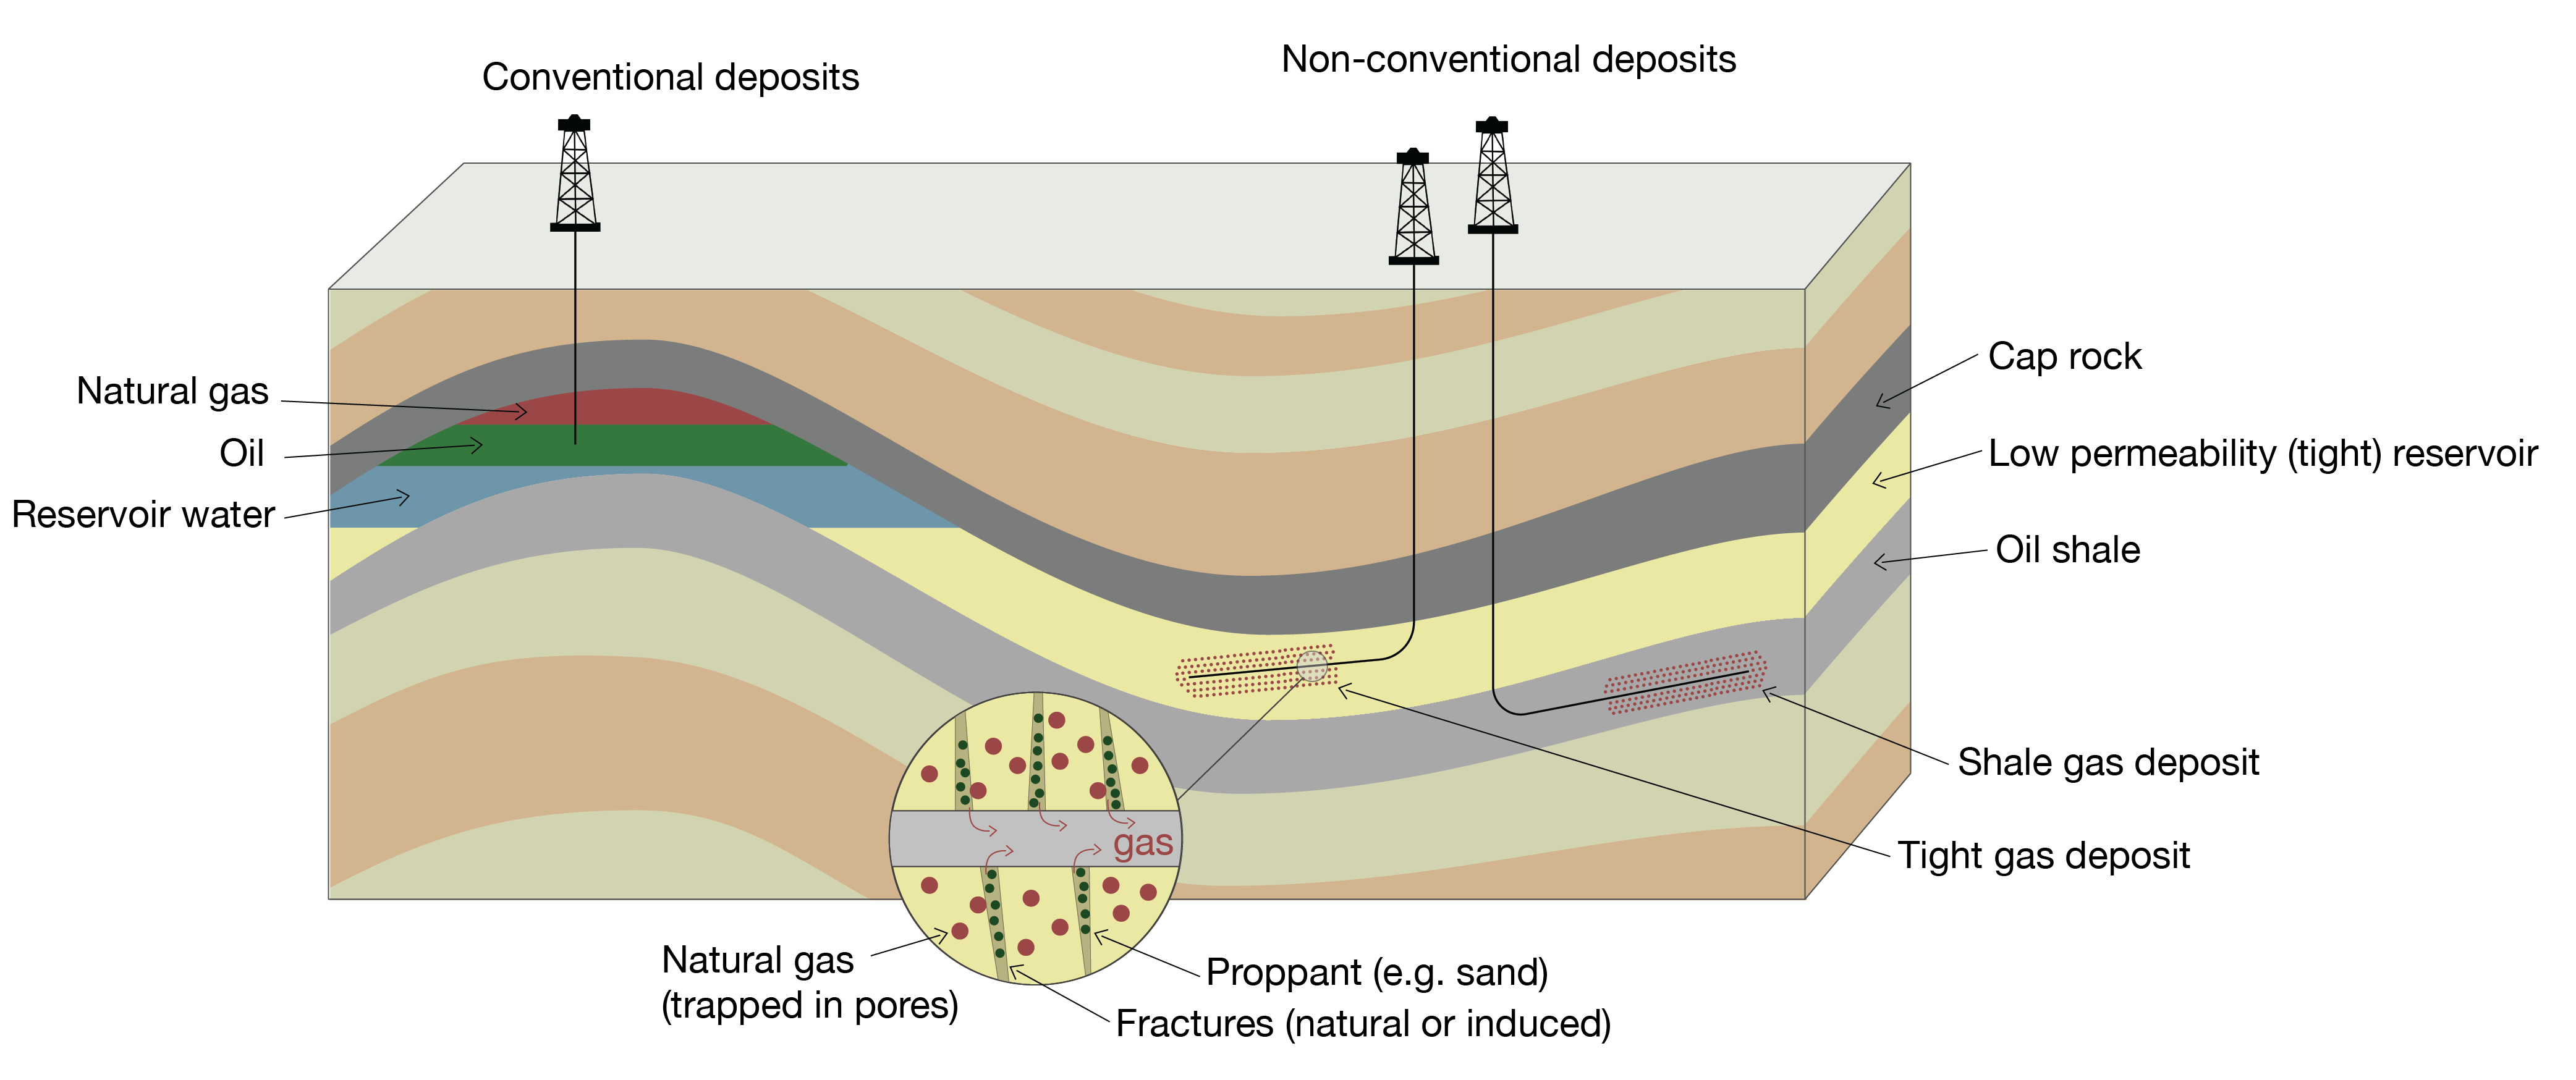
\includegraphics[width=\textwidth]{figures/intro/nonconventional_resources.png}
    \end{center}
\caption{
    Conventional reservoirs contain oil and gas that have migrated upwards
    under pressure until they are trapped by a cap rock (left), while
    non-conventional tight or shale oil and gas reservoirs contain hydrocarbons
    that are trapped in low permeability formations (right).
}
\label{fig:nonconventional_resources}
\end{figure}


To accomplish this task, I propose to use electromagnetic (EM) geophysical techniques. For EM to be a viable method for imaging the distribution of proppant and fluid within a fractured volume of rock, we require that: (1) the fractured volume of rock have physical properties which are distinct from the background, host rock, (2) the survey must be sensitive to this contrast, and (3) once the data have been collected, they must be interpreted or inverted in a meaningful manner. Note that this is a time-lapse problem; that is, by inducing a fracture, the physical properties of the reservoir have been altered. In order to characterize such a change, we must view the imaging problem as a time-lapse one, and collect data to provide us with a before and an after data-view of the reservoir.

Variations in subsurface electrical conductivity have been used as a diagnostic physical property in sedimentary settings for characterizing geologic formations, and the properties and distribution of fluids within those formations. Hydrocarbons are much more resistive than saline formation fluids. In enhanced oil recovery projects, fluids are injected into the formation, which may be less resistive than the hydrocarbons they replace. These contrasts have been the target of cross-well, surface-to-borehole and borehole-to-surface electromagnetic (EM) methods for reservoir monitoring and characterization applications (cf. \cite{Bevc1991, Wilt1995, marsala2008, marsala2011, Marsala2014}).

In the case of hydraulic fracturing, the physical properties of the fractured volume of the reservoir depend upon the properties of the injected fluid and proppant particles. Saline water may be used, as is often the case when recycled water is used, and electrically conductive proppant may be manufactured and injected \citep{cannan2014electrically, Vengosh2014, King2010}. One or both of these may be used to create a physical property contrast between the host reservoir rock and the fractured volume of the reservoir. This contrast is what we aim to excite using an electromagnetic survey.

Using additives to make a hydraulic fracture a geophysical target is not a new idea. \cite{Byerlee1976} suggested using magnetic particles and a magnetic survey to estimate fracture orientation at distances larger than can be determined by tracers and well logs. To create a fracture with a significant magnetic susceptibility, they suggested using finely crushed magnetite suspended in the fracturing fluid or iron shot, spherical particles of iron which do not crush easily and have a high magnetic susceptibility. They treated the fracture as a plate with a known magnetic susceptibility and collected measurements before and after the fracture operation; measurements of the horizontal magnetic field inside of the injection borehole are used to indicate the orientation of the fracture and surface measurements are used to estimate the fracture geometry. Using an analytic model for the magnetic response of a circular disc in a uniform inducing field, they demonstrated the potential of this technique for simple analog models of two fields sites: an engineered geothermal project at Los Alamos, where fractures are induced to circulate fluid through a dry geothermal reservoir and a hydraulic fracture operation for a tight-gas reservoir at Rio Blanco.

Similarly, \cite{Bartel1976} suggest using electrically conductive fracturing fluid and measuring electric potentials at the surface in a DC resistivity experiment where one electrode is connected to the injection well and a return electrode is connected to a distant well casing. Potential electrodes are arranged in two concentric rings centered about the injection well with potential differences being measured between electrodes along the same azimuth in the inner and outer rings. Variations in the amplitude of the potential difference with azimuth are used to estimate the orientation of the fracture and to detect asymmetry (e.g. if the fracture extends further one side of the well than the other). Field tests were performed at two sites and demonstrated detectability of fractures in an experiment in the Wattenburg field for fractures at depths of $\sim$2200m depth. The source electrode was connected to the casing and centered at the depth of the induced fracture (see also \cite{Smith1978}).

Since these initial developments in the late 70's, there have been significant improvements in data quality as well as our ability to model and invert electrical and electromagnetic data in 3D. In conjunction, there have been advancements in fracture operations and imaging techniques such as the use of microseismic, tiltmeters, and pressure-transient analysis to characterize hydraulic fracture. As a result, the questions being asked are more detailed. How complex is the fracture? Is it a simple planar fracture or an extensive network? What is the extent of the propped volume of rock?

To assess if EM can provide insights for helping answer these questions, we need to be able to perform 3D numerical simulations of EM for fractured reservoirs. This prompts a question to be examined in the thesis:
\begin{itemize}
\item{How do we construct a physical property model of a fractured volume of rock that can be used in numerical simulations?}
\end{itemize}

\section{Challenges to electromagnetics with steel-cased boreholes}
\label{sec:challenges-steel-casing}

Hydraulic fracture operations are typically conducted in steel cased wells. These wells presents several significant challenges for modelling and inverting EM geophysical data. Most wells are cased with carbon steel, which has both a large electrical conductivity ($\sim 5.5\times 10^6$ S/m) and magnetic permeability ($> 50 \mu_0$) \citep{wuhabashy1994}. This is a large contrast compared to  typical geologic settings, which typically have conductivities less than 1 S/m and permeabilities similar to that of free space, $\mu_0$. As a result, the casing will have a significant impact on the behavior of the EM fields and fluxes. The properties of the casing, in particular, magnetic permeability, as well as casing thickness, can vary along the length of the well. They also  depend on the quality of the steel and the state of corrosion; this adds another level of complexity to the situation. Well logging tools, such as that described by \cite{brill2012} have been developed to characterize these variations.

Not only does casing introduce a large, variable, physical property contrast, its geometry and scale add to the difficulty. Well casing is cylindrical in shape, typically $\sim$1cm in thickness, $~10$cm in diameter, and may be extend several kilometers in depth, while the geologic structures we aim to characterize with the geophysical survey have three dimensional variations in electrical conductivity on the scale of hundreds of meters to kilometers. Approaches tailored to accurately modelling the impact of the casing in simple 1D geologic settings may be geometrically incompatible or computationally prohibitive to use when reservoir-scale, three-dimensional geologic structures and targets are included in the conductivity model.

In much of the early literature, the casing was viewed as a nuisance which distorts the EM signals of interest. Distortion of surface direct current (DC) resistivity and induced polarization (IP) data, primarily in hydrocarbon settings, was examined in \citep{Wait1983, Holladay1984, Johnston1987} and later extended to grounded source EM and IP in \citep{Wait1985, Williams1985, Johnston1992}. Also in hydrocarbon applications, well-logging in the presence of steel cased boreholes is motivation for examining the behavior of electromagnetic fields and fluxes in the vicinity of casing. Initial work focussed on DC resistivity with \citep{Kaufman1990, Schenkel1990, Kaufman1993, Schenkel1994}, and inductive source frequency domain experiments with \citep{Augustin1989}. \cite{Kaufman1990} derives an analytical solution for the electric field at DC in an experiment where an electrode is positioned along the axis of an infinite-length well. The mathematical solutions presented show how, and under what conditions, horizontal currents leak into the formation outside the well. Moreover, \cite{Kaufman1990} showed, based upon asymptotic analysis, which fields to measure inside the well so that information about the formation resistivity could be obtained. This analysis is extended to include finite-length wells in \cite{Kaufman1993}. \cite{Schenkel1994} show the importance of considering the length of the casing in borehole resistivity measurements, and demonstrate the feasibility of cross-well DC resistivity. They also show that the presence of a steel casing can improve sensitivity to a target adjacent to the well. In frequency domain EM, \cite{Augustin1989} consider a loop-loop experiment, where a large loop is positioned on the surface of the earth and a magnetic field receiver is within the borehole. Magnetic permeability is included in the analysis and a ``casing correction'', effectively a filter due to the casing on inductive-source data, is introduced. This work was built upon for considering cross-well frequency domain EM experiments \citep{Uchida1991, Wilt1996}.

For larger scale geophysical surveys, steel cased wells have been used as ``extended electrodes.'' \cite{Rocroi1985} used a pair of well casings as current electrodes for reservoir characterization in hydrocarbon applications. In near-surface settings \citep{Ramirez1996, Rucker2010, Rucker2012} considered the use of monitoring wells as current and potential electrodes for a DC experiment aimed at imaging nuclear waste beneath a leaking storage tank. Similarly, \cite{Ronczka2015} considers the use of groundwater wells for monitoring a saltwater intrusion and investigates numerical strategies for simulating casings as long electrodes. Imaging hydraulic fractures has been a motivator for a number of studies at DC or EM, among them \cite{Weiss2016, hoversten2017borehole}. Some of these have suggested the use of casings that include resistive gaps so that currents may be injected in a segment of the well and potentials measured across the other gaps along the well \citep{Nekut1995, Zhang2018}.

There has also been an increase in interest in examining the use of electrical or electromagnetic methods deployed on the surface to non-invasively look for flaws or breaks in the casing. \cite{Wilt2018} introduces the idea of using electrical or electromagnetic methods for casing integrity which is further expanded upon in \cite{Wilt2018a}. They show that low-frequency electromagnetic methods are sensitive to variations in wellbore length and demonstrate that their numerical simulations agree with field data collected over two different wellbores at the Containment and Monitoring Institute (CaMI) field site in southern Alberta, Canada. This work provides motivation for further delving into the physics and assessing under which circumstances we can expect to detect a flaw along a wellbore using electrical or electromagnetic methods.

As computing resources increased, our ability to forward-simulate more complex scenarios has improved. However, the large physical property contrasts and disperate length scales introduced when a steel cased well is included in a model still present computational challenges. Even the DC problem, which is relatively computationally light, has posed challenges; those are exacerbated when solving the full Maxwell equations in the frequency (FDEM) or time domain (TDEM) and can become crippling for an inversion. For models where the source and borehole are axisymmetric, cylindrical symmetry may be exploited to reduce the dimensionality, and thus the number of unknowns, in the problem (e.g. \cite{Pardo2013, Heagy2015}).

To reduce computational load in a 3D simulation, a number of authors have employed simplifying assumptions. Several authors replaced the steel-cased well with a solid borehole, either with the same conductivity as the hollow-cased well (e.g. \cite{Um2015, Puzyrev2017}) or preserving the cross sectional conductance (e.g. \cite{Swidinsky2013, Kohnke2017}), so that a coarser discretization may be used; \cite{Haber2016} similarly replaces the borehole with a coarser conductivity structure and adopts an OcTree discretization locally refine the mesh around the casing. \cite{Yang2016} uses a circuit model and introduces circuit components to account for the steel cased well in a 3D DC resistivity experiment; \cite{Weiss2017} adopts a similar strategy in a Finite Element scheme. Another approach has been to replace the well with an ``equivalent source'', for example, a collection of representative dipoles, inspired from \cite{cuevas2014}, or with linear charge distributions for a DC problem \citep{Weiss2016}. For the frequency domain electromagnetic problem, a method of moments approach, which replaces the casing with a series of current dipoles, has been taken in \cite{Kohnke2017}.

For 3D survey geometries, only a handful of forward simulations which accurately discretize the casing have been demonstrated, and they have been achieved at significant computational cost. Recent examples, including \cite{Commer2015, Um2015, Puzyrev2017}, perform time and frequency domain simulations with finely-discretized boreholes; they required the equivalent of days of compute-time for a single forward simulation to complete. While these codes will undoubtedly see improvements in efficiency, there remains a need to accurately discretize the casing at modest computational cost both to serve as tool which these codes can compare against as well as a need for researchers to be able to interact with and explore the behavior of the currents, charges, electric and magnetic fields and fluxes to develop an understanding of the physics in these high-contrast settings.

There are a host of research questions to be explored in the context of highly conductive, permeable, steel cased wells in electromagnetic applications. This thesis is concerned with developing an understanding of the physics of electromagnetics in settings with steel cased wells. In order to delve into the physics, we must have a mechanism for simulating Maxwell's equations which raises the question:
\begin{itemize}
\item{How do we develop a numerical approach that allows us to sufficiently discretize the steel casing so that we can not only simulate DC and EM data, but also explore the finer details of the currents, charges, electric and magnetic fields?}
\end{itemize}

Assuming a numerical strategy can be developed, we can then begin to explore questions about the physics. At the DC limit,
\begin{itemize}
\item{How do the currents, charges and electric fields behave in settings with steel cased wells? What are the implications for survey design?}
\item{Are there physical insights which, when incorporated into numerical algorithms, reduce the computational cost of simulations with steel-cased wells?}
\end{itemize}

Finally, electromagnetic experiments introduce the complication of time-variation in the fields and fluxes as well as the additional concern of variable magnetic permeability in the model. Though the influence of the magnetic permeability of steel-casings has been explored for inductive source EM (e.g. where the source is a circular loop or magnetic dipole) \citep{wuhabashy1994}, the influence of magnetic permeability on grounded-source EM surveys (e.g. where two electrodes are used to inject current into the earth, similar to a DC resistivity experiment) is relatively unexplored. This prompts questions like:
\begin{itemize}
\item{How do the fields and fluxes behave in an EM experiment which includes a steel-cased well?}
\item{What impact does magnetic permeability have on the behavior of the fields and fluxes? How important is it to consider in numerical simulations?}
\end{itemize}

These questions will serve as motivation for three chapters on steel-cased wells in the thesis.

\section{Research motivation and thesis structure}
The common theme throughout the thesis is the motivation to image subsurface injections -- specifically proppant and fluid injected during a hydraulic fracturing operation. To this end, I consider three main topics that comprise five chapters in the thesis:
\begin{itemize}
    \item{Building a physical property model for a fractured volume of rock (Chapter \ref{ch:phys-prop-model})}
    \item{Developing a physical understanding of electrical and electromagnetic methods when steel-cased wells are present (Chapter \ref{ch:casing-software}, \ref{ch:casing-dc}, and \ref{ch:casing-em})}
    \item{Formulating and solving the inverse problem for a fractured volume of rock (Chapter \ref{ch:inversion})}
\end{itemize}
Each of these topics is discussed in further detail below.

The research chapters in this thesis make use of fundamental knowledge that needs to be presented. Rather than insert that introductory material into the individual chapters, they are included at the end of this chapter. The background elements pertain to:
\begin{itemize}
\item{Electromagnetic geophysics: introducing Maxwell's equations and EM geophysical surveys}
\item{Geophysical inversions: formulating the inverse problem}
\end{itemize}
These are successively presented in Sections \ref{sec:background-em} and \ref{sec:background-inversions} after I have introduced the research material in this thesis.

\subsection{Homogenization strategy for hydraulic fractures}
Chapter \ref{ch:phys-prop-model} develops a strategy for estimating a bulk conductivity of a fractured volume of rock. I break the problem into two steps, first estimating the effective conductivity of a mixture of electrically conductive proppant and fluid and second, estimating the conductivity of a fractured volume of rock where the fractures are filled with the proppant-fluid mixture. Having constructed a physical property model for a modest-sized fracture operation, I then demonstrate feasibility of detecting EM signal sensitive to the fracture using a well-established cross-well EM survey. At this stage, I neglect the influence of steel-cased wells.

The homogenization strategy taken in this chapter is based on established methods in effective medium theory \citep{Bruggeman1935} which have previously been considered for fractured rocks \citep{Berryman2013}. The main contributions of this chapter are: algorithmic improvements to the effective conductivity calculation presented by \cite{Berryman2013}, and the discussion of the two-stage workflow which allows various proppant-fluid mixtures to be considered (e.g. a fully conductive proppant-pack, mixture of standard sand or ceramic proppant and conductive proppant).


\subsection{Steel casings}

The intention in this thesis is to advance our understanding of the physics of EM in settings with steel-cased wells. This understanding can then be used to develop appropriate approximations in order to reduce computational cost, and to help calibrate our expectations of the results of more advanced numerical techniques. To this end, I consider three topics, each corresponding to one chapter in the thesis, to advancing our physical understanding.

Chapters \ref{ch:casing-software}, \ref{ch:casing-dc}, and \ref{ch:casing-em} contend with some of the challenges of performing DC and EM surveys in settings with steel-cased wells. In Chapter \ref{ch:casing-software}, I present a mimetic finite volume implementation for simulating Maxwell's equations at DC, in frequency and in time, on cylindrically symmetric and 3D cylindrical meshes (which include an azimuthal discretization). Although cylindrically symmetric meshes are common in EM modelling, cylindrical meshes which include an azimuthal discretization are not. A cylindrical mesh conforms to the geometry of a vertical borehole and thus, can greatly reduce the size of the mesh, and resultant cost of the computation, while still allowing for significant refinement in the vicinity of the borehole. The purpose of this implementation is to facilitate investigation into the physical behavior of EM fields and fluxes in this high-contrast setting. I consider two forms of validation: numerical validation and validation of the physical behavior. For numerical validation, I compare results of a forward simulation with independently developed codes \citep{Haber2007, Commer2015, Yang2016}. For validation of the physical behavior, I compare features of the simulated currents, charges, and electric fields to the behavior expected from the asymptotic analysis in \cite{Kaufman1990, Kaufman1993} at DC, and similarly, compare the behavior of the magnetic fields and fluxes in the presence of conductive and permeable pipes with the lab studies and analytical work contained in \cite{Augustin1989} for inductive source frequency-domain electromagnetics.

Chapter \ref{ch:casing-dc} focuses on developing an understanding of the physics of casings in a DC resistivity experiment. I start by considering the related application of casing integrity. In a casing integrity experiment, the aim is to detect a flaw or break in the casing which might be due to corrosion or failure under mechanical stresses. Wellbore integrity surveys are typically conducted with wireline tools, but more recently, \cite{Wilt2018} introduced the idea of conducting a survey from the surface. This application provides the opportunity to build a physical understanding about the behavior of the currents, charges, and electric fields in a DC experiment with casing. I investigate factors that influence the feasibility of detecting a flaw, including the conductivity of the background and casing, depth to the flaw, and impact on the signal if the whole circumference or only a portion of the circumference of the casing is compromised. I also consider the location of the return electrode and its impact on the measured data. Many of the concepts developed in this section inform survey design elements in the next section, which considers DC resistivity survey for a conductive or resistive target adjacent to the well. I look at survey design elements, including the impact of the source electrode location on the resultant currents over the depth-interval of interest, and consider the impact of parameters such as the conductivity of the target and whether the target is electrically connected to the casing or not. The final topic in this chapter considers approximations to the steel-cased well in order to reduce the computational cost of the forward model. There is discrepancy among current literature as to whether the contrast between the background and the casing is the important quantity to conserve (e.g. \cite{Um2015}) or if the product of the conductivity and the cross-sectional area of the casing should be preserved (e.g. \citep{Swidinsky2013}). I compare both approaches to resolve this question and discuss implications of choosing an incorrect approximation.

Chapter \ref{ch:casing-em} explores important aspects of electromagnetics in settings with steel cased well. I begin by demonstrating the behavior of currents through time in time-domain EM simulation with a conductive well. The geometry of the currents through time is rather complex, even in this seemingly simple experiment. Building from this, I then consider magnetic permeability and demonstrate how permeability alters the behavior of the currents and in turn, discuss the impact permeability can have on data measured at the surface. Finally, I revisit approaches for approximating steel cased wells developed at DC and explore some of the subtleties that arise in EM experiments.
\subsection{Inversions for subsurface injections}
Chapter \ref{ch:inversion} returns to the application of hydraulic fracturing and examines the inverse problem for a fractured volume of rock. Using a DC resistivity experiment, I explore both voxel-based and parametric strategies for extracting information about the fractured volume of rock. These inversions demonstrate some of the challenges caused by steel cased wells and their influence on the sensitivity. Finally, I demonstrate how effective medium theory can be incorporated into the inversion and frame the inverse problem as an inversion for fracture concentration. This alters the sensitivity and provides the opportunity to incorporate a constraint on the volume of injected proppant and fluid.
\subsection{Appendices}
The thesis additionally includes 5 Appendices. Appendix \ref{app:code_list} provides a listing of the source code used to perform all of the examples shown in the thesis. Following this, there are two technical appendices, Appendix \ref{app:concentric_spheres} and \ref{app:scemt-derivs}, which support content in Chapters \ref{ch:phys-prop-model} and \ref{ch:inversion}, respectively. Appendix \ref{app:simpegem} describes the open-source software used in this thesis to simulate and invert Maxwell's equations. The final appendix, Appendix \ref{app:education}, discusses how the open-source software development practices adopted in this thesis and the broader SimPEG community are similarly used for the development of interactive educational resources for geophysics in the GeoSci.xyz project (\href{https://geosci.xyz}{https://geosci.xyz}).

\subsection{A note on reproducibility and dissemination}

Although simulating and inverting data in settings with steel-cased wells has practical applications, within the realm of geophysics, and even within EM geophysics, it is a narrow topic. The value in focussing on specific applications is that each application has its own subtleties and tangible details that must be worked through. In their own right, the discoveries that are made by working through these details are of value to the application-at-hand. However, this does not have to be the limit of their impact. If you choose to take the perspective that the problem-at-hand is an instance of a larger class of research questions, this allows you to view the methods and software needed to make incremental scientific discoveries as reusable components. It is then worth the investment of effort to develop and refactor these pieces so that they are modular building blocks that fit into a larger framework and are of use to a broader community. This is the perspective I have sought to take as I conducted the research described in this thesis.

The simulations and inversions build on and contribute to the SimPEG framework, which is described in \cite{Cockett2015, Heagy2017, Cockett2017}. SimPEG is written in python and is open-source, licensed under the permissive MIT license. Source code for all of the examples shown are also openly licenced and are available on GitHub as a combination of python scripts and Jupyter notebooks. Each chapter has a corresponding code-repository; Appendix \ref{app:code_list} provides a summary of where these can be accessed. My intention in providing all of the source-code is to be transparent about the work completed; in addition, I hope these developments are of use and value to the broader geophysics community.
\section{Background: Electromagnetic geophysics}
\label{sec:background-em}
Before moving into the research content of the thesis, I will provide a brief overview of the governing equations in electromagnetics and recommend \cite{Ward1988} and \cite{emgeosci} for more in-depth discussion on the physics. For an overview of how to numerically solve Maxwell's equations, I refer the reader to \cite{Haber2014}.
\subsection{Governing equations}
The equations which govern the physics of EM are Maxwell’s equations:
\begin{equation}
\begin{split}
    \nabla \times \vec{e} + \frac{\partial \vec{b}}{\partial t} &= 0 \\
    \nabla \times \vec{h} - \frac{\partial \vec{d}}{\partial t} &= \vec{j}
\end{split}
\label{eq:maxwell_time_full}
\end{equation}

where $\vec{e}$ is the electric field (V/m), $\vec{b}$ is the magnetic flux density (T), $\vec{h}$ is the magnetic field (A/m), $\vec{d}$ is the electric displacement (C/m$^2$), $\vec{j}$ is the current density (A/m$^2$). The first equation is Faraday’s law; it describes how a time-varying magnetic flux generates rotational electric fields. The second equation is the Ampere-Maxwell equation (Maxwell's contribution was the addition of the displacement current term, $\partial \vec{d} / \partial t$). It describes how a currents generate rotating magnetic fields.

It is sometimes also convenient to consider Maxwell’s equations in the frequency domain. Using the $e^{i\omega t}$ Fourier transform convention and capital letters to denote variables in the frequency domain, Maxwell’s equations are given by
\begin{equation}
\begin{split}
    \nabla \times \vec{E} + i \omega\vec{B} &= 0 \\
    \nabla \times \vec{H} - i \omega\vec{D} &= \vec{J}
\end{split}
\label{eq:maxwell_freq_full}
\end{equation}


These partial differential equations are coupled through the constitutive relations which relate the fields and fluxes through physical properties:
\begin{equation}
\begin{split}
\vec{J} &= \sigma \vec{E} \\
\vec{B} &= \mu \vec{H} \\
\vec{D} &= \varepsilon \vec{E}
\end{split}
\label{eq:constitutive_relations_full}
\end{equation}
.
where $\sigma$ is electrical conductivity (S/m), $\mu$ is magnetic permeability (H/m), and $\varepsilon$ is the dielectric permittivity (F/m). Electrical conductivity varies over many orders of magnitude; two examples on the extreme ends are the conductivity of air, $\sim10^{-8}$ S/m and the conductivity of steel, $\sim 10^6$ S/m. The reciprocal of electrical conductivity is resistivity ($\rho = 1/\sigma$), which has units of $\Omega$m. Throughout the thesis, resistivity and conductivity will be used interchangeably. The value of magnetic permeability is often taken to be that of free-space, $\mu_0 = 4\pi\times10^{-7}$ H/m, in geophysical electromagnetic applications, as the permeability of most earth-materials ranges from 1-10 $\mu_0$ \citep{Telford1990}. The permeability of steel, however, is $\sim 100 \mu_0$, thus for settings with steel-cased wells, the simplifying assumption that $\mu=\mu_0$ cannot necessarily be invoked. The value of dielectric permittivity varies between the free-space value of $\varepsilon_0=8.85\times10^{-12}$ F/m and the dielectric permittivity of water, $80\varepsilon_0$ \citep{Telford1990}. Variations in dielectric permittivity are relevant at high frequencies, such as those used in ground penetrating radar (GPR) surveys (> $10^5$ Hz), but in most geophysical electromagnetic surveys, late-time or low frequencies are employed as the high-frequencies signals attenuate rapidly in conductive earth-materials. As such, the quasi-static approximation, which neglects displacement currents (the $\partial \vec{d} / \partial t$-term in equation \ref{eq:maxwell_time_full} and the $i\omega\vec{D}$ term in equation \ref{eq:maxwell_freq_full}), is commonly adopted, and will be used throughout the thesis. Under the quasi-static assumption, Maxwell’s equations are given by:
\begin{equation}
\begin{split}
    \nabla \times \vec{e} &= -\frac{\partial \vec{b}}{\partial t} \\
    \nabla \times \vec{h}  &= \vec{j}
\end{split}
\label{eq:maxwell_time_quasi}
\end{equation}

in time, and:
\begin{equation}
\begin{split}
    \nabla \times \vec{E} &= -i \omega\vec{B}  \\
    \nabla \times \vec{H} &= \vec{J}
\end{split}
\label{eq:maxwell_freq_quasi}
\end{equation}

 in frequency.

In the electrostatic limit, the time-derivative terms vanish. Taking the divergence of Ampere's law, and recognizing that the electric field $\vec{e}$ is curl-free and can therefore be expressed as the gradient of a scalar potential $\phi$, gives us the governing equations for the DC resistivity problem:
\begin{equation}
\begin{split}
\nabla \cdot \vec{j} &= I\left(\delta(\vec{r} - \vec{r}_{s^{+}}) - \delta(\vec{r} - \vec{r}_{s^{-}})\right) \\
\vec{e} &= - \nabla \phi
\end{split}
\label{eq:dc_equations}
\end{equation}

Here $\vec{j}$ is the current density, $I$ is the magnitude of the source current, and $\vec{r}_{s^+}$ and $\vec{r}_{s^-}$ are the location of the positive and negative source electrodes, respectively. The electric field and the current density are related through Ohm’s law (the first equation in equation \ref{eq:constitutive_relations_full}), which we can invoke to reduce the two first-order partial differential equations in equation \ref{eq:dc_equations} to a single, second order equation in $\phi$:
\begin{equation}
\nabla \cdot \sigma \nabla \phi = - I\left(\delta(\vec{r} - \vec{r}_{s^{+}}) - \delta(\vec{r} - \vec{r}_{s^{-}})\right)
\label{eq:dc_equation_second_order}
\end{equation}

This poisson equation can be solved for the electric potential, $\phi$, from which values of the currents and electric fields can be directly computed. In addition to considering the current density and electric fields, I will also present results in terms of charges throughout the thesis. The charge density is related to the electric field through
\begin{equation}
\nabla \cdot \vec{e} = \frac{\rho_f}{\varepsilon_0}
\label{eq:charge_density}
\end{equation}


\subsection{Geophysical surveys}
To generate data, we require that a source be used to excite a response and that receivers measure the resultant fields and/or fluxes. In order to excite a response, a source is needed. Sources can be natural, plane-wave sources, as in the case of the magnetotelluric method, or they can be controlled, man-made sources. Broadly speaking, two categories of controlled sources exist: inductive sources and grounded sources. Inductive sources consist of a loop of wire through which a time-varying current is passed, this in turn generates time-varying magnetic fields which act as the source fields, as shown in an Airborne EM example in Figure \ref{fig:inductive-sources}. The time-varying magnetic field created by these systems induces currents in the conductive earth which, in turn, create secondary magnetic fields which can be measured at or above the surface. Within reservoir settings, cross-well EM is a commonly applied inductive source survey \citep{Wilt1995}.


\begin{figure}
    \begin{center}
    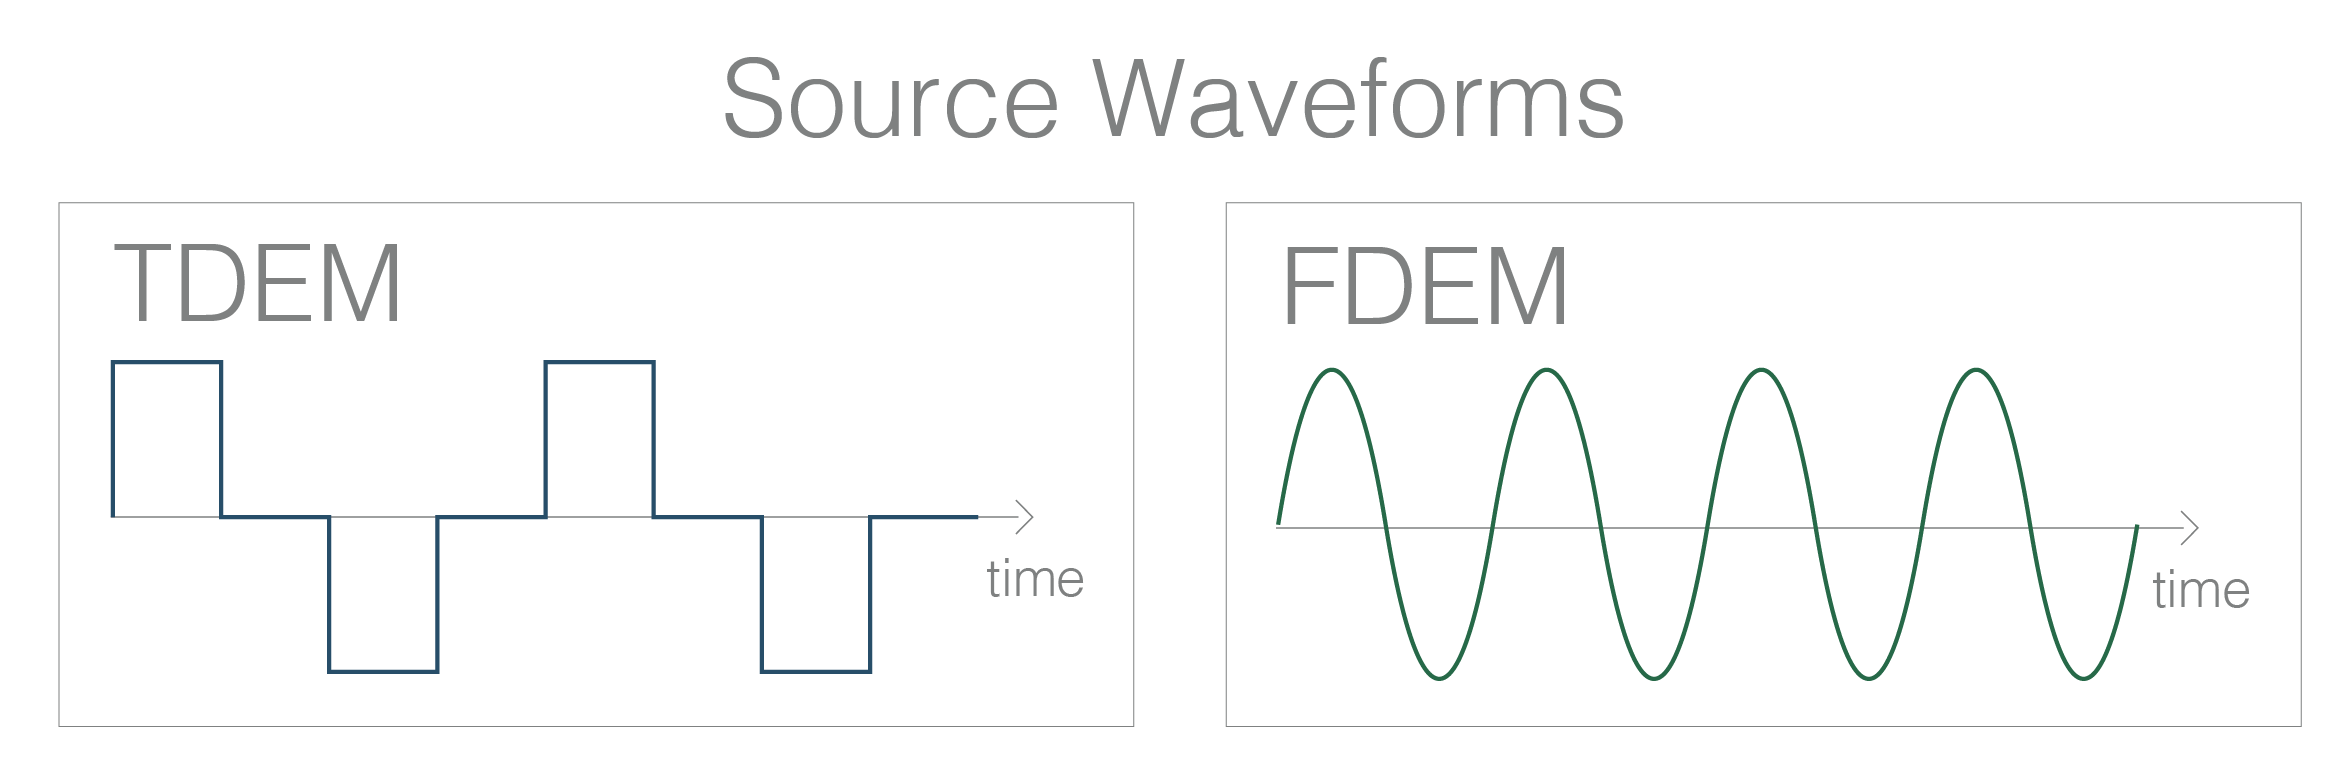
\includegraphics[width=0.7\textwidth]{figures/intro/waveforms.png}
    \end{center}
\caption{
    The choice of whether to solve the EM equations in the time-domain (TDEM) or the frequency domain (FDEM) depends upon the transmitter waveform; a step-off-type waveform (left) lends itself to a solution approach in the time domain and a harmonic signal (right) is typically addressed in the frequency domain.
}
\label{fig:waveforms}
\end{figure}



\begin{figure}
    \begin{center}
    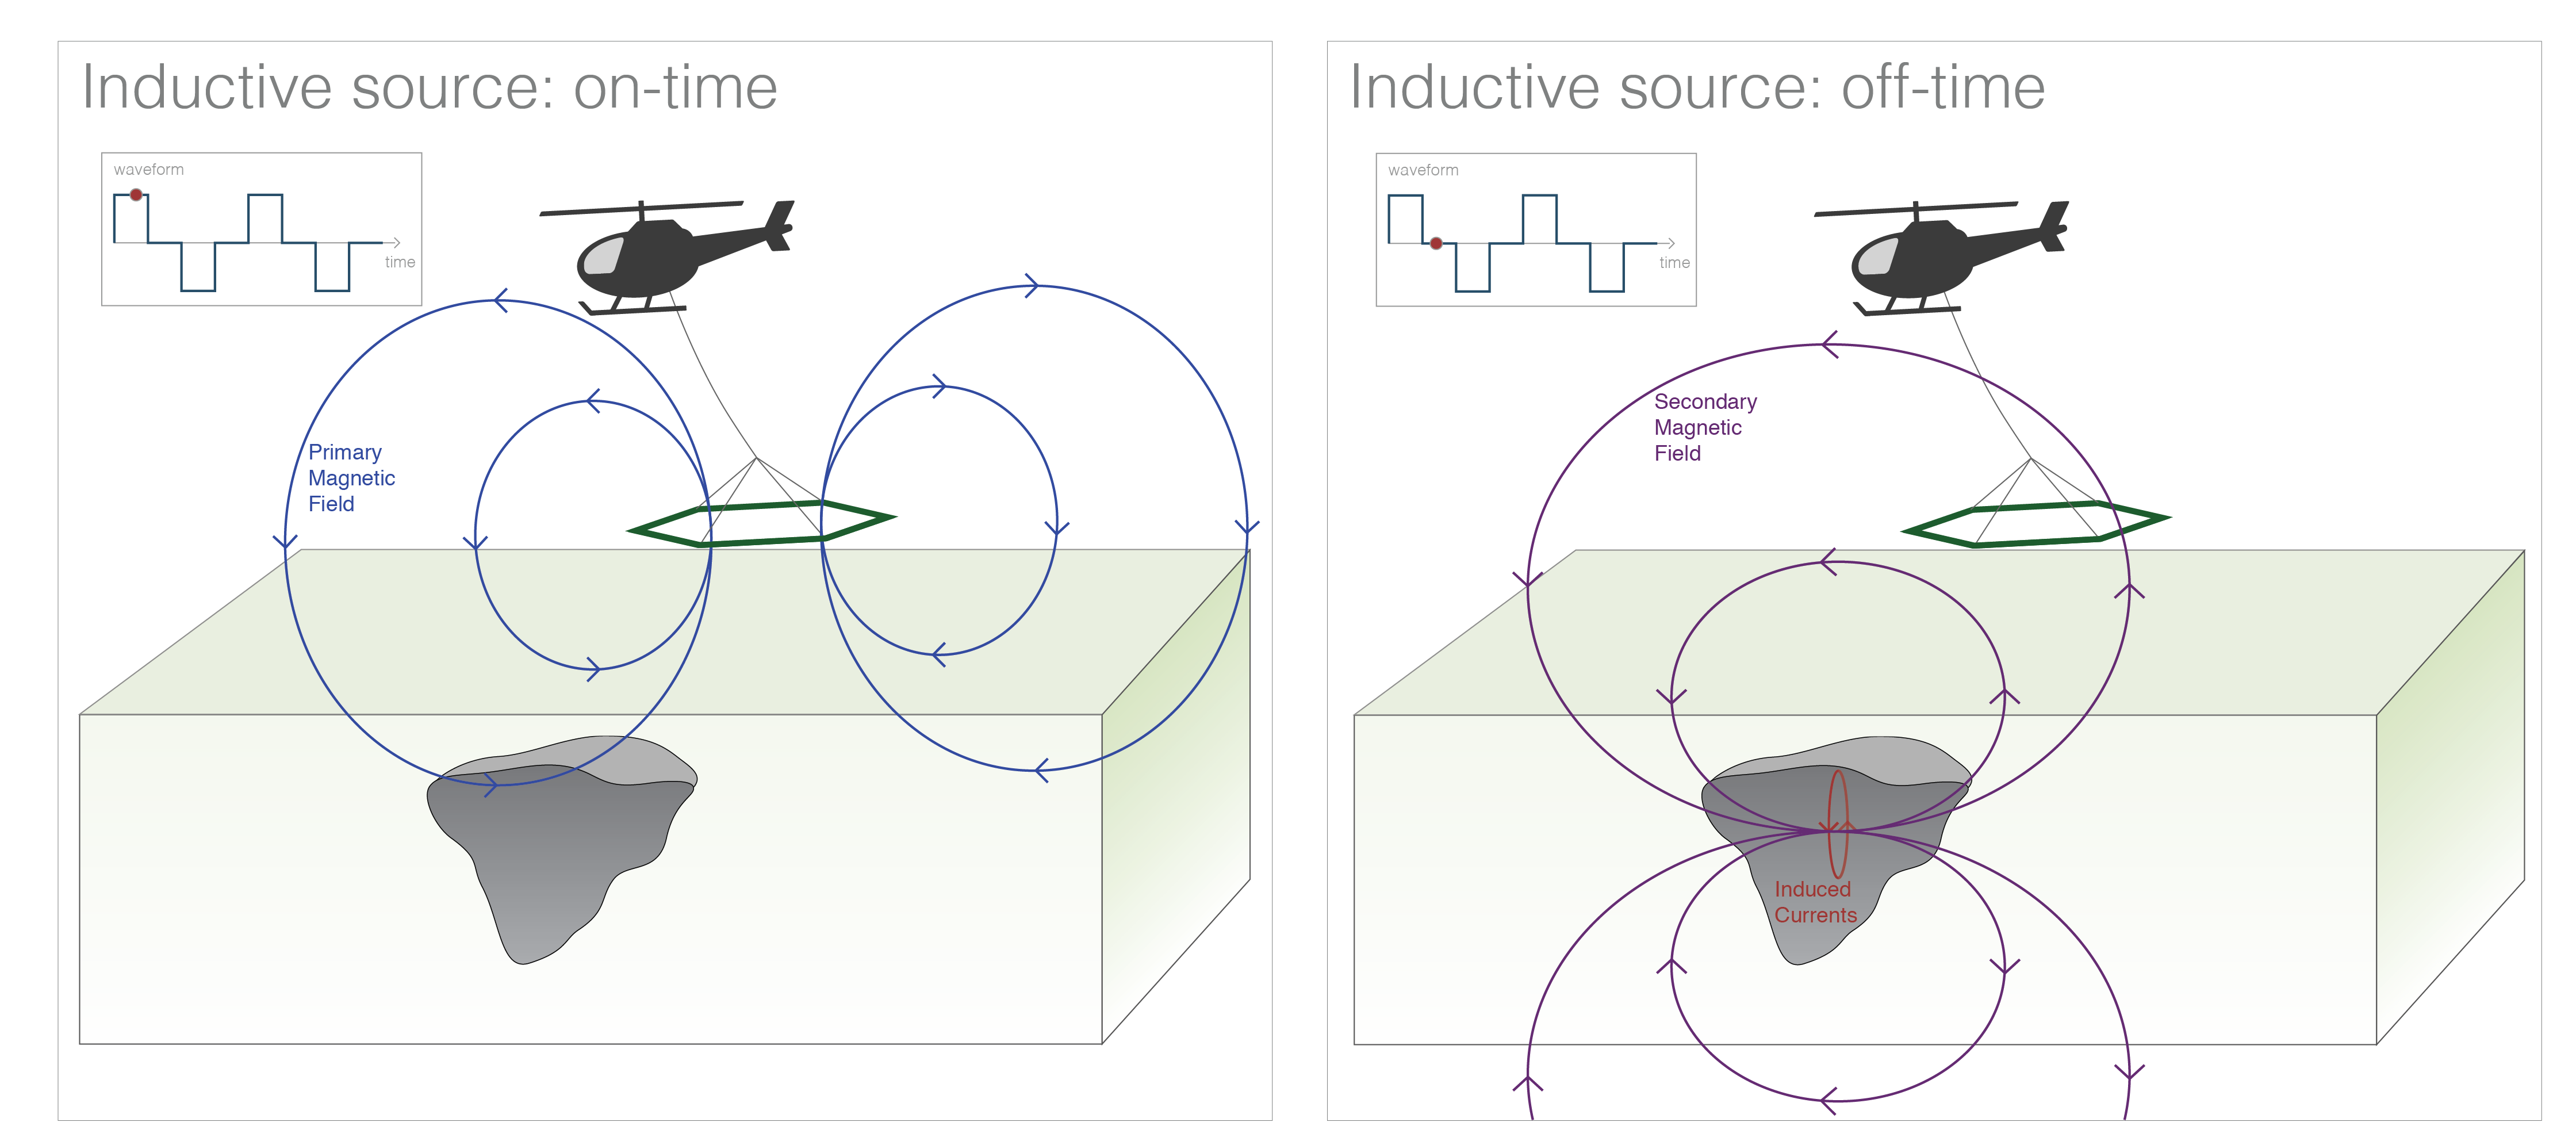
\includegraphics[width=\textwidth]{figures/intro/inductive-sources.png}
    \end{center}
\caption{
    Time-domain inductive source experiment. (Left) a steady-state current is passed through the transmitter loop, generating a primary magnetic field. (Right) This current is shut-off, causing a change in magnetic flux. The changing magnetic flux induces secondary currents in conductors, which in turn create secondary magnetic fields that can be measured at receivers above, on, or within the earth.
}
\label{fig:inductive-sources}
\end{figure}


Grounded sources require an electrical connection between the source and the earth. Two electrodes are positioned on, or in, the ground, the positive electrode injects current and a return electrode is a current-sink, as shown in Figure \ref{fig:grounded-sources}. In the electrostatic limit, a grounded-source experiment is simply a DC resistivity experiment. Galvanic currents flow through the earth and cause charges to build up at conductivity interfaces, generating electric potentials which can be measured at the surface or within boreholes. Electromagnetics introduces a time-varying component. The time-varying current flowing through the wire generates a time-varying primary magnetic field. This induces vortex currents in conductive structures within the earth. Receivers can measure electric fields, magnetic flux, or time-variations in the magnetic flux or some combination of these.

\begin{figure}
    \begin{center}
    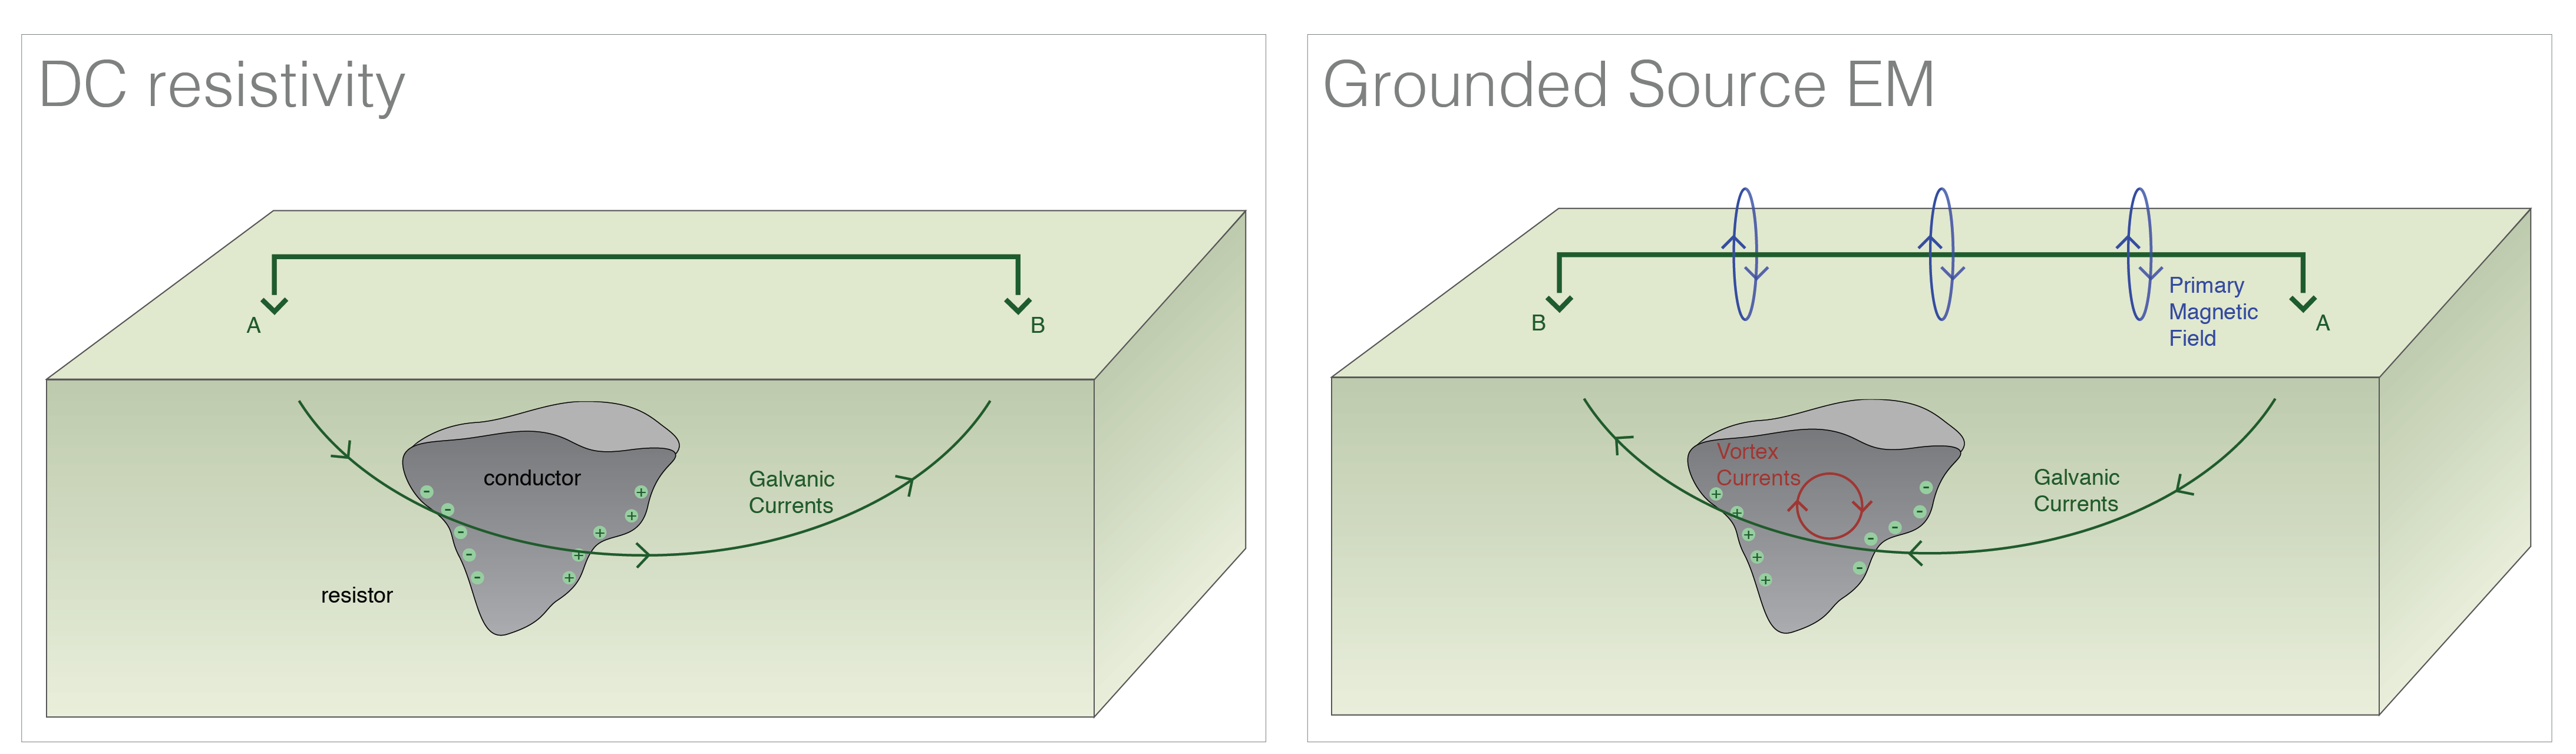
\includegraphics[width=\textwidth]{figures/intro/grounded-sources.png}
    \end{center}
\caption{
    (Left) Direct current resistivity experiment in which a steady-state current is injected into the earth, and
    (Right) a grounded source electromagnetic experiment which uses a time-varying source current.
}
\label{fig:grounded-sources}
\end{figure}


Two things are needed to generate data that are sensitive to a target or structure of interest. First, the source must be capable of getting EM energy to the target to excite a response, and second, the response must reach the receivers with sufficient amplitude to be measurable. A measurable signal is one which is (a) above the noise floor of the receivers, and (b) comprises a significant percentage of the primary (that is, the response with no target present). Numerical simulation of Maxwell's equations is a critical component for assessing feasibility of detecting a target, and is an essential element of the inverse problem in which we aim to estimate a model from measured data. Within the thesis, I discuss the machinery used to perform numerical simulations in Chapter \ref{ch:casing-software} and in Appendix \ref{app:simpegem}.
\section{Background: Geophysical Inversions}
\label{sec:background-inversions}

Once data have been collected, an inverse problem can be formulated. The goal of the inversion is to extract information about the subsurface from the data. Formulating, implementing and solving the inverse problem can be viewed as a workflow consisting of inputs, implementation, and evaluation, as shown in Figure \ref{fig:inversion_workflow_bullets}. The inputs are composed of the data, the governing equations, and prior knowledge or assumptions about the setting. In the case of the fracturing problem, this may include well-log resistivity measurements which provide information about the background, knowledge of where the fracture was initiated, and the volumes of proppant and fluid pumped to create the fracture.
The implementation consists of two broad categories: the forward simulation and the inversion. The forward simulation is the means by which we solve the governing equations given a model, and the inversion components evaluate and update this model. I consider a gradient based approach, which updates the model through an optimization routine. The output of this implementation is a model, which, prior to interpretation, must be evaluated. This requires considering, and often re-assessing, the choices and assumptions made in both the input and implementation stages (c.f. \cite{Oldenburg2005, Haber2014a, Cockett2015}).

\begin{figure}
    \begin{center}
    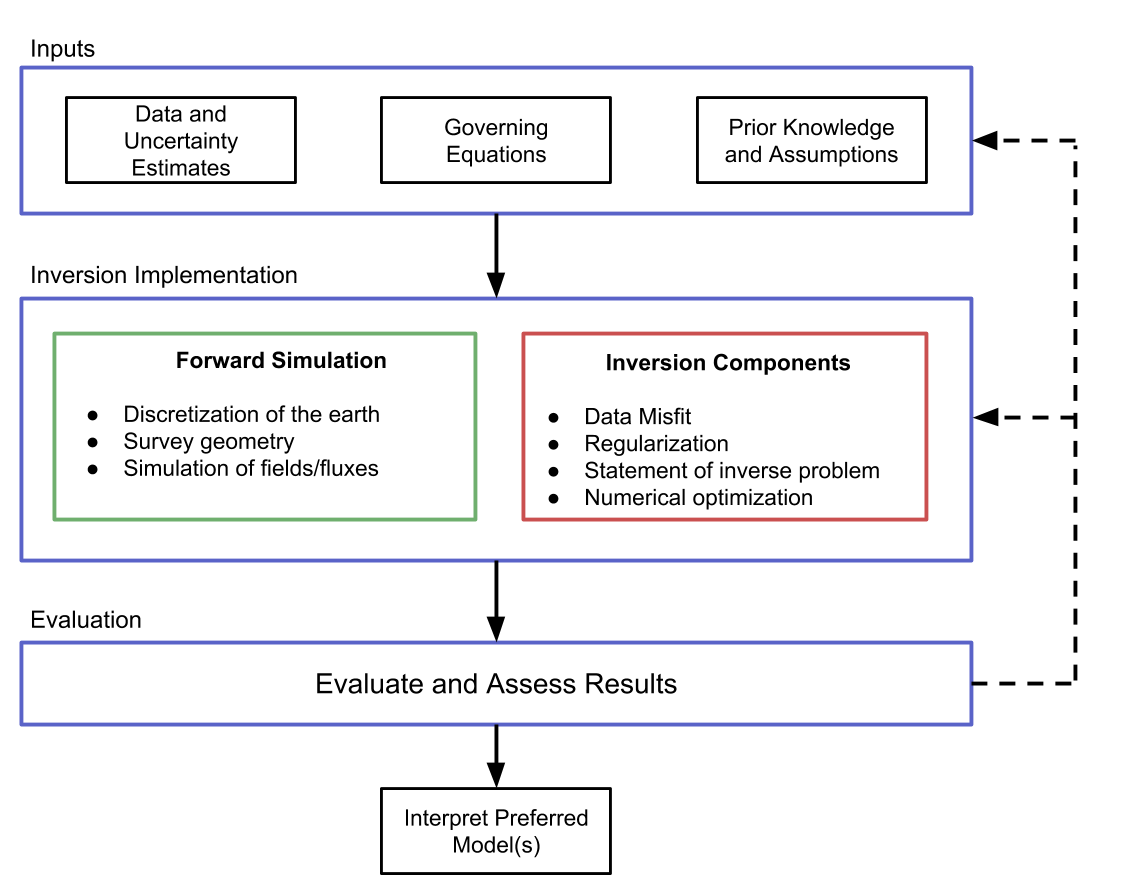
\includegraphics[width=\textwidth]{figures/intro/inversion_workflow_bullets.png}
    \end{center}
\caption{
    Overview of a geophysical inversion workflow. Adapted from \cite{Cockett2015}.
}
\label{fig:inversion_workflow_bullets}
\end{figure}


\subsection{Formulating and solving the inverse problem}
In this section, I provide a brief overview of geophysical inversions, adapted from \cite{Cockett2015}; for more detail and examples, the reader is reffered to \cite{Oldenburg2005, Cockett2015} as well as Appendix \ref{app:simpegem} for details specific to forward and inverse modelling in electromagnetics.

The aim of a geophysical inversion is to use the collected data to extract information about the subsurface. In a given survey, a datum can be written as
\begin{equation}
F_i[\mathbf{m}] + \epsilon_i = d_i
\label{eq:geophysical_datum}
\end{equation}

where $F[\cdot]$ is the forward simulation operator; for an electromagnetic problem, it simulates Maxwell’s equations given a source and samples the relevant fields and fluxes at the receiver locations. The physical properties of the subsurface are captured by the variable $m$, which I refer to as the inversion model. The noise is described by $\epsilon_i$, and $d_i$ is the observed datum. A survey usually includes multiple sources and receivers, resulting in the observed data $\mathbf{d}_{\rm obs} = [d_1, ... , d_N]$ and some estimate of their uncertainties -- often assumed to be Gaussian. If the noise is Gaussian, then an appropriate measure of the data misfit is the $l_2$-norm of the difference between the predicted data obtained through a forward simulation and the observed data, namely
\begin{equation}
\phi_{\rm d}(\mathbf{m}) = \frac{1}{2}\|\mathbf{W}_{\rm d}(F[\mathbf{m}] - \mathbf{d}_{\rm obs})\|^2
\label{eq:data_misfit}
\end{equation}

$\mathbf{W}_{\rm d}$ is a diagonal matrix whose elements are equal to $\mathbf{W}_{\rm d_{ii}}=1/\epsilon_i$ where $\epsilon_i$ is an estimated standard deviation of the $i$\textsuperscript{th} datum. A good option is to assign a $\epsilon_i = floor + \%|d_i|$.
Percentages are generally required when there is a large dynamic range of the data. A percentage alone can cause great difficulty for the inversion if a particular datum acquires a value close to zero, and therefore we include a floor.

In addition to a metric that evaluates the size of the misfit, it is also required that we have a tolerance, $\phi_d^*$; models satisfying $\phi_d(\mathbf{m}) \leq \phi_d^*$ are considered to adequately fit the data \citep{Parker1994}. If the data errors are Gaussian and we have assigned the correct standard deviations, then the expected value of $\phi_d^* \sim N/2$, where $N$ is the number of data. Note that the division by 2 is because the statement of the data misfit includes the factor of 1/2 to simplify derivatives. When describing the ``data-fit'' of an inversion, it is common to quote a $\chi$-factor, which is defined as
\begin{equation}
\phi_d^{\rm inv} = \chi\phi_d^*
\label{eq:chi-factor}
\end{equation}

Where $\phi_d^{\rm inv}$ is the final data-misfit in the inversion.  Finding a model that has a misfit substantially lower than this will result in a solution that has excessive and erroneous structure, that is, we are fitting the noise. Finding a model that has a misfit substantially larger than this will yield a model that is missing structure that could have been extracted from the data (see \cite{Oldenburg2005} for a tutorial).

The goal of an inversion is to estimate the earth-model, $m$ from the data. In reality, the physical property distribution of the subsurface is continuous; therefore, estimating this model from a finite number of data is an ill-posed problem, meaning no unique model explains the data. Thus, in order to obtain a meaningful model from the data, assumptions and additional information must be included. There are several mechanisms by which this can be achieved. One of the most common is to include consideration of a model regularization, $\phi_m$ in the inverse problem. This norm can penalize variation from a reference model, spatial derivatives of the model, or some combination of these. For example, the Tikhonov-style regularization function can be expressed as
\begin{equation}
\phi_{\rm m}(\mathbf{m}) =
    \frac{\alpha_s}{2}\|\mathbf{W}_{\rm s}(\mathbf{m} - \mathbf{m}_{\rm ref})\|^2 +
    \frac{\alpha_x}{2}\|\mathbf{W}_{\rm x}\mathbf{m}\|^2 +
    \frac{\alpha_y}{2}\|\mathbf{W}_{\rm y}\mathbf{m}\|^2 +
    \frac{\alpha_z}{2}\|\mathbf{W}_{\rm z}\mathbf{m}\|^2
\label{eq:model_regularization}
\end{equation}

The first term is referred to as the ``smallness'' and penalizes difference between the inversion model and a reference model $\mathbf{m_{\rm ref}}$. The matrix $\mathbf{W}_s$ is a diagonal matrix; in the simplest case it is the identity matrix. The remaining three terms are the first-order smoothness in the x, y, and z directions; the matrices $\mathbf{W}_{\rm x}$, $\mathbf{W}_{\rm x}$, $\mathbf{W}_{\rm y}$ and $\mathbf{W}_{\rm z}$ approximate the first order spatial derivatives in each direction. The $\alpha$ parameters weight the relative contribution of each term to the regularization. Their values should consider the length-scales in the problem (c.f. \cite{Oldenburg2005}); for a typical 3D problem $\alpha_x = \alpha_y = \alpha_z = 1$ and $\alpha_s$ is generally chosen to be several orders of magnitude smaller than the smoothness weights.

To define the inverse problem, I take a deterministic approach to the inversion and treat it as an optimization problem. Additional strong constraints on the model such as upper and lower bounds ($\mathbf{m}_u$, $\mathbf{m}_l$) are also considered. The general form of the objective function I use combines the data misfit and regularization with a trade-off parameter, $\beta$, between them, giving a problem of the form
\begin{equation}
\begin{split}
&\underset{\mathbf{m}}{\text{minimize}} \quad \phi(\mathbf{m}) = \phi_d(\mathbf{m}) + \beta \phi_m(\mathbf{m}) \\
&\text{such that} \quad \phi_d \leq \phi_d^*, \quad \mathbf{m}_l \leq \mathbf{m} \leq \mathbf{m}_u
\end{split}
\label{eq:inverse_problem}
\end{equation}

Since the value of $\beta$ is not known \emph{a priori}, the above optimization problem can be solved at many values of $\beta$ to produce a trade-off, or Tikhonov, curve (cf. \cite{Parker1994}). An optimum value, $\beta^*$, can be found so that solving equation \ref{eq:inverse_problem} with $\beta^*$ produces a model with misfit $\phi_d^*$. One approach to finding the value of $\beta^*$ is to use cooling techniques where the $\beta$ is progressively reduced from some high value and the process stopped when the tolerance is reached.

The optimization problem posed in equation \ref{eq:inverse_problem} is non-linear for DC resistivity and electromagnetic forward simulations requiring that iterative optimization techniques be employed (c.f. \cite{Nocedal1999}). Gradient-based techniques are commonly employed. In particular, Gauss-Newton methods are effective in geophysical inversions. To ease notation, I consider a more compact description of the model regularization, and write our objective function as
\begin{equation}
\phi(\mathbf{m}) = \frac{1}{2}\|\mathbf{W}_{\rm d}(F[\mathbf{m}] - \mathbf{d}_{\rm obs})\|^2 + \frac{\beta}{2}\|\mathbf{W}_{\rm m}\mathbf{m}\|^2
\label{eq:objective_function}
\end{equation}

Note that if $\mathbf{m}_{\rm ref} = \mathbf{0}$ and $\mathbf{W}_{\rm m} = [\mathbf{W}_{\rm s}^\top, \mathbf{W}_{\rm x}^\top, \mathbf{W}_{\rm y}^\top, \mathbf{W}_{\rm z}^\top]^\top$, then the regularization is equivalent to that stated in equation \ref{eq:model_regularization}. The gradient is given by
\begin{equation}
\mathbf{g}(\mathbf{m})=
    J[\mathbf{m}]^\top \mathbf{W}_{\rm d}^\top \mathbf{W}_{\rm d}(F[\mathbf{m}]-\mathbf{d}_{\rm obs})
    + \beta \mathbf{W}_{\rm m}^\top \mathbf{W}_{\rm m} (\mathbf{m})
\label{eq:objective_function_gradient}
\end{equation}

where $J[\mathbf{m}]$ is the sensitivity or Jacobian. The components $J[\mathbf{m}]_{ij}$ specify how the $i$\textsuperscript{th} datum changes with respect to the $j$\textsuperscript{th} model parameter,
\begin{equation}
    J[\mathbf{m}] = \frac{d F[\mathbf{m}]}{d \mathbf{m}}
\label{eq:sensitivity}
\end{equation}

I discuss the derivation of the sensitivity for time and frequency domain electromagnetic problems in depth in Appendix \ref{app:simpegem}.

At the $k$\textsuperscript{th} iteration, beginning with a model $\mathbf{m}^{k}$, we search for a perturbation $\delta \m$ that reduces the objective function. Linearizing the forward simulation by Taylor expansion,
\begin{equation}
F[\mathbf{m}^{k}+\delta \mathbf{m}] \simeq F[\mathbf{m}^{k}] + \mathbf{J}[\mathbf{m}^{k}]\delta \mathbf{m} + \mathcal{O}(\delta \mathbf{m})^2
\label{eq:taylor_expand_forward_simulation}
\end{equation}


and setting the gradient equal to zero yields the standard Gauss-Newton equations
to be solved for the perturbation $\delta \mathbf{m}$:
\begin{equation}
(J[\mathbf{m}]^\top \mathbf{W}_{\rm d}^\top \mathbf{W}_{\rm d} J[\mathbf{m}] + \beta \mathbf{W}_{\rm m}^\top \mathbf{W}_{\rm m}) \delta \mathbf{m} = -\mathbf{g}(\mathbf{m})
\label{eq:gauss_newton}
\end{equation}

The updated model is given by
\begin{equation}
\mathbf{m}^{k+1}=\mathbf{m}^{k} + \gamma \delta \mathbf{m}
\label{eq:model_update}
\end{equation}

where $\gamma \in (0,1]$ is a coefficient that can be found by a line search.
Setting $\gamma=1$ is the default and a line search is necessary if $\phi(\mathbf{m}^{k+1}) \ge \phi(\mathbf{m}^{k})$.

The iterative optimization process is continued until a suitable stopping criterion is reached.
Completion of this iterative process yields a minimization for particular value of the trade-off parameter, $\beta$. If we are invoking a cooling schedule, and if the desired misfit tolerance is not yet achieved, $\beta$ is reduced and the iterative numerical optimization procedure is repeated.

The forward simulation, computation of the sensitivities, and inversion machinery that I use throughout this thesis are implemented in the open source software package, SimPEG \citep{Cockett2015, Heagy2017}.


